\section{Das Teilchen im Kasten}
\authors{Atousa Seyedian, Ole Simmering}

\subsection{Allgemein}

Das Modell des Teilchens im Kasten ist ein eindimensionales Modell, welches als Näherung einer chemischen Bindung aufgefasst werden kann. In dem Kasten wird die potentielle Energie für $ 0 \leq x \leq L $ mit null gleich gesetzt.
Hier gilt also $ V_x = 0 $. 
Der Kasten ist begrenzt von Wänden an den $ x $-Werten $ x = 0 $ und $ x=L $. Außerhalb des Kastens ist das Potential unendlich (siehe Abbildung \ref{Potential im Kasten}).


\begin{dsafigure}
 \centering
 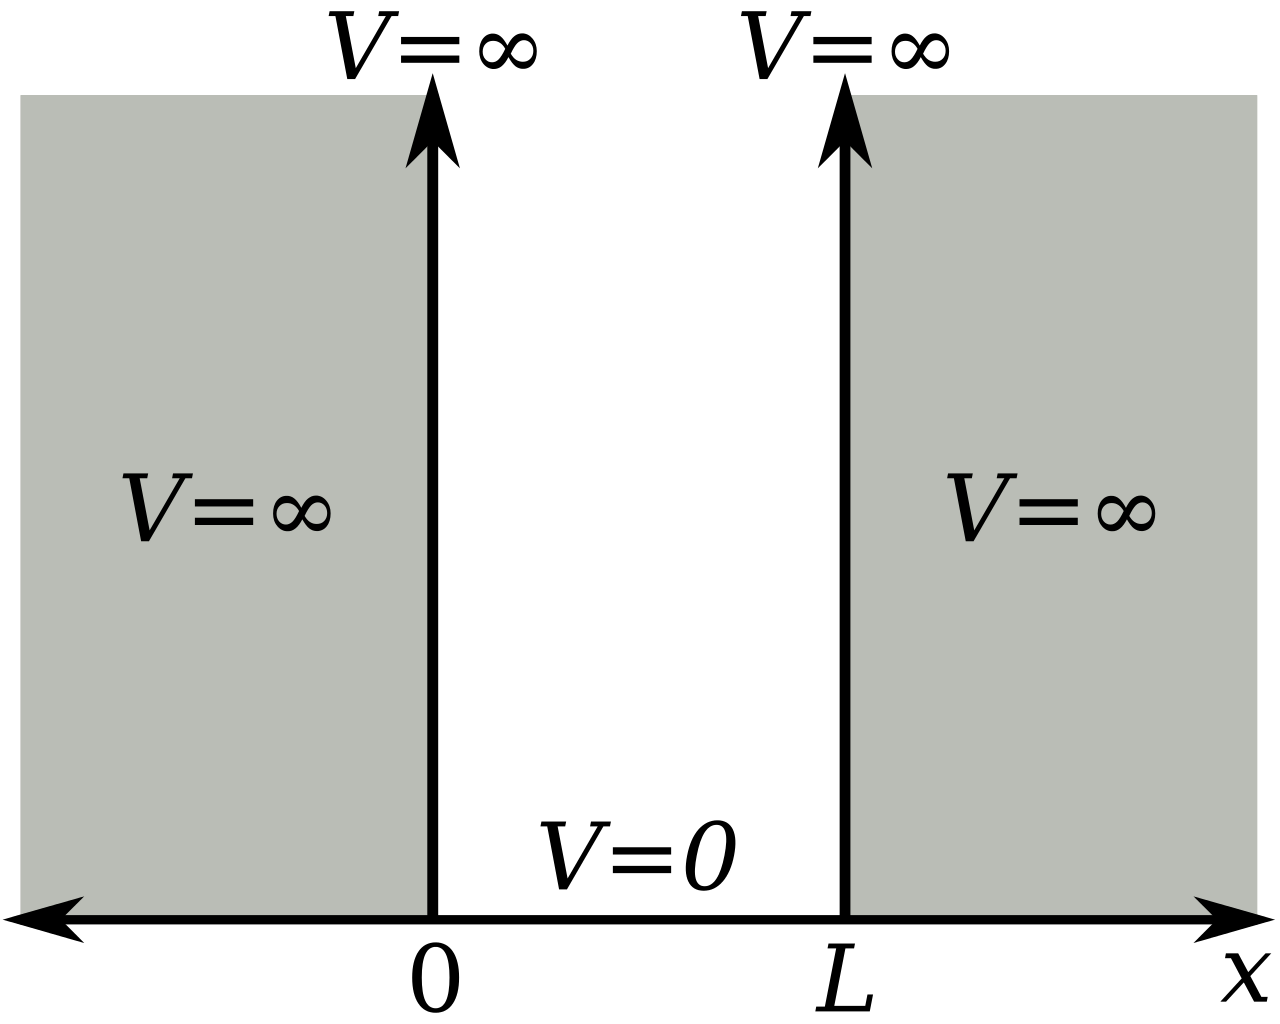
\includegraphics[width=\columnwidth]{potential_kasten.png}
 \caption{Darstellung des Potentials im Modell des Teilchens im Kasten.
\cite{wikiKastenpot}}
 \label{Potential im Kasten}
\end{dsafigure} 

Die allgemeine Form der Schrödinger Gleichung lautet $ E\psi=\hat{H}\psi $. Der Hamilton-Operator $ \hat{H} $ ist der Operator für die kinetische und potentielle Energie eines Teilchens $ \hat{H}=\hat{T}+\hat{V} $. Da im Modell die potentielle Energie innerhalb des Kastens verschwindet, lässt sich der Hamilton Operator mit dem Operator der kinetischen Energie gleich setzen: $ \hat{H}=\hat{T} $. Damit lautet die Schrödingergleichung \cite{Atkins2001}:
\begin{equation}
E \psi = - \dfrac{\hbar ^2}{2m} \dfrac{d^2}{dx^2}\psi  
\end{equation}
 

Ein möglicher Ansatz für die Wellenfunktion ist $ \psi (x) = A \cdot \sin (kx) + B \cdot \cos (kx) $. Da die Wellenfunktion stetig sein muss und die Randbedingungen besagen, dass die Wellenfunktion bei $ x=0 $ und $ x=L$  den Wert $0$ annehmen muss, muss der Parameter $ B $ gleich $0$ gesetzt werden, sodass die Formel nach Einsetzen der Randbedingungen auf $ \psi (x) = A \cdot \sin (kL) $ reduziert werden kann. Dabei muss $ kL $ aufgrund der Randbedingungen ein ganzzahliges Vielfaches von $ n\cdot\pi $ sein. Die Wellenlänge $\lambda $ muss abhängig von der Länge $ L $ des Kastens sein. Es gilt: $ \lambda = n\pi/L $ mit $ n \in \mathbb{N} $. Somit muss $ k=n\pi/L $ sein. Die Wellenfunktion ist nun:
 
\begin{equation}
\psi (x) = A \sin \left(\dfrac{n \pi}{L} x\right)
\end{equation}
    
und nach Normierung:

\begin{equation}
\psi(x)=\sqrt{\dfrac{L}{2}}\sin \left(\dfrac{n \pi x}{L}\right). 
\end{equation}


Damit kann nun die Schrödingergleichung gelöst werden. Die Energien der verschiedenen Niveaus sind: 

\begin{equation}
E_n = \frac{\hbar^2 \pi^2 n^2}{2m L^2} = \frac{h^2 n^2}{8m L^2}
\end{equation}



\subsection{Farbigkeit von Molekülen}

Das Teilchen im Kasten ist eine grobe Näherung, die zur Berechnung von Anregungsenergien von Molekülen genutzt werden kann. Die dafür benötigte Energiedifferenz beträgt $ \Delta E = E_{n+1}-E_n $, wobei $ n $ das obersten besetzten Energieniveau ist. Diese Energie muss der des eingestrahlten Lichtes entsprechen, um das Molekül anzuregen.
